\documentclass{article}
\usepackage[english]{babel}
\usepackage[letterpaper,top=2cm,bottom=2cm,left=3cm,right=3cm,marginparwidth=1.75cm]{geometry}
\usepackage{amsmath}
\usepackage{graphicx}
\usepackage{algorithm2e}
\usepackage{forest}
\usepackage[colorlinks=true, allcolors=blue]{hyperref}

\title{\textbf{CS456: Algorithm Design and Analysis}}
\author{Elikem Asudo Tsatsu Gale-Zoyiku}
\date{\today}

\begin{document}
\maketitle
\begin{center}
    \begin{large}
        \textbf{Assignment 3\\}
    \end{large}
\end{center}
\newpage
\section*{Question 1}
\subsection*{Recursive Calls of Partition Method}
List: \[Q, U, E, B, R, A, C, H, O\]

When the pivot is List[0] == Q:

\[ [A, E, B, C, H, O], [Q], [U, R] \]

For sublist \([A, E, B, C, H, O]\) with pivot Left[0] == A:
\[ [A], [E, B, C, H, O] \]

For sublist \([E, B, C, H, O]\) with pivot Right[0] == E:
\[ [B, C], [E], [H, O] \]

For sublist \([B, C]\) with pivot Left[0] == B: \[ [B], [C] \]

For sublist \([H, O]\) with pivot Right[0] == H: \[ [H], [O] \]

For sublist \([U, R]\) with pivot Right[0] == U: \[ [R], [U] \]

\subsection*{List After Each Partition Call}
After Each Call of Partition Method:

\[
    [Q, U, E, B, R, A, C, H, O]
\]

\[
    [A, E, B, C, H, O], [Q], [U, R]
\]

\[
    [A], [E, B, C, H, O], [Q], [U, R]
\]

\[
    [A], [B, C], [E], [H, O], [Q], [U, R]
\]

\[
    [A], [B], [C], [E], [H,], [O], [Q], [U], [R]
    \textit{(singletons so recursive calls end)}\]

Sorted list: \[ [A, B, C, E, H, O, Q, R, U] \]
\newpage
\section*{Question 2}
Analyzing the running times of each algorithm:

\subsection*{Algorithm A}
\begin{itemize}
    \item Divides the problem of size \( n \) into 5 subproblems of size \( n/2 \).
    \item Recursively solves each subproblem.
    \item Combines the solutions in linear time.
\end{itemize}

The recurrence relation for Algorithm A can be expressed as:
\[
    T(n) = 5T(n/2) + O(n)
\]
\[ A = 5, B = 2, k = 1, p = 0, and A > b^{k}\]
By using the Master Theorem, the time complexity of Algorithm A is \( O(n^{\log_b{a}}) \) == \( O(n^{\log_2{5}}) \) which is equivalent to
\( O(n^{2.322}) \)

\subsection*{Algorithm B}
\begin{itemize}
    \item Divides the problem of size \( n \) by recursively solving two subproblems of size \( n - 1 \)
    \item Combines the solutions in constant time.
\end{itemize}

The recurrence relation for Algorithm B can be expressed as:
\[ T(n) = 2T(n-1) + O(1) \]

Solving the recurrence relation using substitution:

\[
    \begin{aligned}
        T(n) & = 2T(n-1) + O(1)                                               \\
             & = 2[2T(n-2) + O(1)] + O(1)                                     \\
             & = 2^2 T(n-2) + 2O(1) + O(1)                                    \\
             & = 2^3 T(n-3) + 2^2 O(1) + 2O(1) + O(1)                         \\
             & = \cdots                                                       \\
             & = 2^k T(n-k) + 2^{k-1} O(1) + \cdots + 2^2 O(1) + 2O(1) + O(1)
    \end{aligned}
\]

At each step, the problem size \( n \) reduces by 1, so \( n - k = 1 \) when \( k = n - 1 \) (base case).\\

When \( k = n - 1 \):
\[ T(n) = 2^{n-1} T(1) + 2^{n-2} O(1) + \cdots + 2^2 O(1) + 2O(1) + O(1) \]

\( T(1) \) is a constant because only the constant time portion of the relation will remain when \( n = 1 \). \\

Thus, T(1) is denoted as \( c \).

\[ T(n) = 2^{n-1} c + 2^{n-2} O(1) + \cdots + 2^2 O(1) + 2O(1) + O(1) \]

In this expression, the dominant term is \( 2^{n-1} c \). Dropping the lower-order terms and constants, \\

the time complexity of Algorithm B:

\[ T(n) = O(2^{n-1}) = O(2^n) \]

Therefore, the time complexity of Algorithm B is \( O(2^n) \).

\subsection*{Algorithm C}
\begin{itemize}
    \item Divides the problem of size \( n \) into nine subproblems of size \( n/3 \).
    \item Recursively solves each subproblem.
    \item Combines the solutions in \( O(n^2) \) time.
\end{itemize}

The recurrence relation for Algorithm C can be expressed as:
\[
    T(n) = 9T(n/3) + O(n^2)
\]
\[ A = 9, B = 3, k = 2, p = 0, and A == b^{k}\]\\


By using the Master Theorem, the time complexity of Algorithm C is \( O(n^{k}) \) == \( O(n^2) \).

\subsection*{Comparison of Time Complexities}
\begin{itemize}
    \item Algorithm A has a time complexity of \( O(n^{\log_2{2.322}}) \).
    \item Algorithm B has a time complexity of \( O(2^n) \).
    \item Algorithm C has a time complexity of \( O(n^2) \).
\end{itemize}

Algorithm C has the lowest time complexity of \( O(n^2) \). \\

Therefore, Algorithm C would be the preferred choice for solving the problem of size \( n \).
\newpage
\section*{Question 3}
\subsection*{a}
\subsection*{Algorithm for Identifying the Heavier Ball in a Group of 9 Balls}

\begin{itemize}
    \item First Iteration: Divide the 9 balls into three groups of three balls each.

          \begin{itemize}
              \item Step 1: Place three balls on each side of the weighing scale.
              \item Step 2: If the scale tips to one side, it indicates that the heavier ball is in that group of three. If the scale remains balanced, the heavier ball is among the remaining three balls.
              \item Step 3: Take the group of three balls that contains the heavier ball (if any) and set the other six balls aside.
          \end{itemize}

          Since there are three balls on each side of the scale, there are only two possible outcomes: one side is heavier, indicating that the heavier ball is among those three balls, or the scale remains balanced, indicating that the heavier ball is among the remaining three balls.

    \item Second Iteration: Divide the three remaining balls into three groups of one ball each.

          \begin{itemize}
              \item Step 1: Place one ball on each side of the weighing scale, leaving one ball aside.
              \item Step 2: If one side of the scale is heavier, it indicates that the heavier ball is among those two balls. If the scale remains balanced, the heavier ball is the one left aside.
          \end{itemize}

          With only three balls remaining, there are only two possible outcomes: one side is heavier, indicating that the heavier ball is among those two balls, or the scale remains balanced, indicating that the heavier ball is the one left aside.

\end{itemize}
\subsection*{b}
\subsection*{Algorithm for Identifying the Heavier Ball in a Group of N Balls where N is a perfect power of 3}
To solve this problem where N-1 balls are of exactly the same weight and one ball is heavier, an extended form of the previous algorithm can be used.\\


This technique would divide the balls into three equal groups in each iteration and compare the weights of the groups on the balance:

\begin{itemize}
    \item Initialization:
          \begin{itemize}
              \item Divide the N balls into three equal groups of size N/3 each.
              \item Place one group on each side of the balance, leaving one group aside.
          \end{itemize}

    \item Weighing:
          \begin{itemize}
              \item If the balance tips to one side, it indicates that the heavier ball is among the balls on that side.
              \item If the balance remains balanced, it means the heavier ball is among the balls that were left aside.
          \end{itemize}

    \item Recursion:
          \begin{itemize}
              \item Recursively apply the same process to the group of balls identified as potentially containing the heavier ball.
          \end{itemize}

    \item Base case:
          \begin{itemize}
              \item When the number of balls in a group becomes 1, that ball is the heavier one.
          \end{itemize}

    \item Termination:
          \begin{itemize}
              \item The process terminates when, in each iteration, N is a perfect power of 3.
              \item The number of iterations needed to find the heavier ball is logarithmic with base 3.
              \item Therefore, the number of times the balance will be weighed is approximately log3(N).
          \end{itemize}
\end{itemize}

\begin{algorithm}[H]
    \SetAlgoLined
    \SetKwInOut{Input}{Input}
    \SetKwInOut{Output}{Output}


    \Input{N balls, where N is a perfect power of 3}
    \Output{The index of the heavier ball}

    \SetKwFunction{IdentifyHeavierBall}{IdentifyHeavierBall}

    \SetKwProg{Fn}{Function}{:}{}

    \Fn{\IdentifyHeavierBall{balls}}{
        \If{length of balls is 1}{
            \Return the index of that single ball as it will be the heavier ball\;
        }
        \begin{itemize}
            \item Divide the balls into three equal groups of size N/3 each and assign them to groups A, B, and C\;
            \item Place group A on the left side of the balance and group B on the right side, leaving group C aside\;
        \end{itemize}
        \If{the balance tips to the side of A}{
            \IdentifyHeavierBall{group A} The heavier ball is in group A\;
        }
        \ElseIf{the balance tips to the other side}{
            \IdentifyHeavierBall{group B}   The heavier ball is in group B\;
        }
        \Else{
            \IdentifyHeavierBall{group C} The heavier ball is in group C because A and B weigh the same\;
        }
    }

    \IdentifyHeavierBall{N balls}\;

\end{algorithm}

\subsection*{c}
Let T(N) be the number of weighings needed to find the heavier ball among N balls. Since the algorithm divides the balls into three equal groups in each iteration, and N is a perfect power of 3, the recurrence relation can be expressed as follows:

\[T(N) = T\left(\frac{N}{3}\right) + O(1)\]
This recurrence relation represents the number of weighings needed to find the heavier ball among N balls by recursively applying the same process to the group of balls identified as potentially containing the heavier ball. Each recursion involves dividing the number of balls by 3 and adding some constant time to account for the weighing operation in each iteration.
\\The base case of the recurrence relation occurs when there is only one ball left to be weighed, in which case T(1) = 1, as no additional weighings are needed, and the index of the ball is returned.
\\Therefore, the recurrence relation for the algorithm is:

\[T(N) =
    \begin{cases}
        1                             & \text{if } N = 1 \\
        T\left(\frac{N}{3}\right) + 1 & \text{if } N > 1
    \end{cases}\]


\subsection*{d}
\[T(N) = T\left(\frac{N}{3}\right) + 1\]
\[T\left(\frac{N}{3}\right) = T\left(\frac{N}{9}\right) + 1\]
\[T\left(\frac{N}{9}\right) = T\left(\frac{N}{27}\right) + 1\]
After \(k\) divisions:

\[T\left(\frac{N}{3^k}\right) = T(1) + k\]

Since \(N = 3^k\), \(k\):

\[3^k = N\]

\[k = \log_3(N)\]

Substituting \(k\) back into the expression:

\[T\left(\frac{N}{3^{\log_3(N)}}\right) = T(1) + \log_3(N)\]

\[T(1) = 1\]
Therefore, the closed-form solution for the recurrence relation is:
\[T(N) = \log_3(N) + 1\] equivalent to
\[O(\log_3(N))\]\\
Using induction to prove:\\
\\Base Case:\\
\\When \(N = 1\), \(T(1) = \log_3(1) + 1 = 0 + 1 = 1\)\\
\\This satisfies the base case.\\
\\Inductive Step:
\\Assume that for all \(N' < N\), \(T(N') = \log_3(N') + 1\).
\\
\\Consider \(T(N)\):

\[T(N) = T\left(\frac{N}{3}\right) + 1\]\\
By the inductive hypothesis, we have:

\[T\left(\frac{N}{3}\right) = \log_3\left(\frac{N}{3}\right) + 1\]\\
Hence,

\[T(N) = \log_3\left(\frac{N}{3}\right) + 1 + 1\]

\[T(N) = \log_3(N) - 1 + 1 + 1\]

\[T(N) = \log_3(N) + 1\]
\[T(N) = O(log_3(N))\]\\
This completes the proof by induction.
\newpage
\section*{Question 4}
\subsection*{a}
\begin{algorithm}[H]
    \SetAlgoLined
    \SetKwFunction{FMain}{topologicalSort}
    \SetKwProg{Fn}{Function}{:}{}
    \Fn{\FMain{graph}}{
        \begin{itemize}
            \item Initialize an empty stack $S$ to store vertices in the correct order\;
            \item Mark all vertices as unvisited\;
        \end{itemize}


        \For{each vertex in graph}{
            \If{vertex is unvisited}{
                performDFS(vertex, $S$)\;
            }
        }

        \While{$S$ is not empty}{
            vertex = pop from stack $S$\;
            print vertex\;
        }
    }
    \BlankLine
    initialize an empty stack $S$ to store vertices in the correct order\;
    mark all vertices as unvisited\;

    \For{each vertex in graph}{
        \If{vertex is unvisited}{
            performDFS(vertex, $S$)\;
        }
    }

    \While{$S$ is not empty}{
        vertex = pop from stack $S$\;
        print vertex\;
    }

    \BlankLine
    \SetKwFunction{FMain}{performDFS}
    \SetKwProg{Fn}{Function}{:}{}
    \Fn{\FMain{vertex, $S$}}{
        mark vertex as visited\;

        \For{each neighbor of vertex}{
            \If{neighbor is unvisited}{
                performDFS(neighbor, $S$)\;
            }
        }

        push vertex onto stack $S$\;
    }
\end{algorithm}
\newpage
\subsection*{b}
\begin{figure}[h]
    \centering
    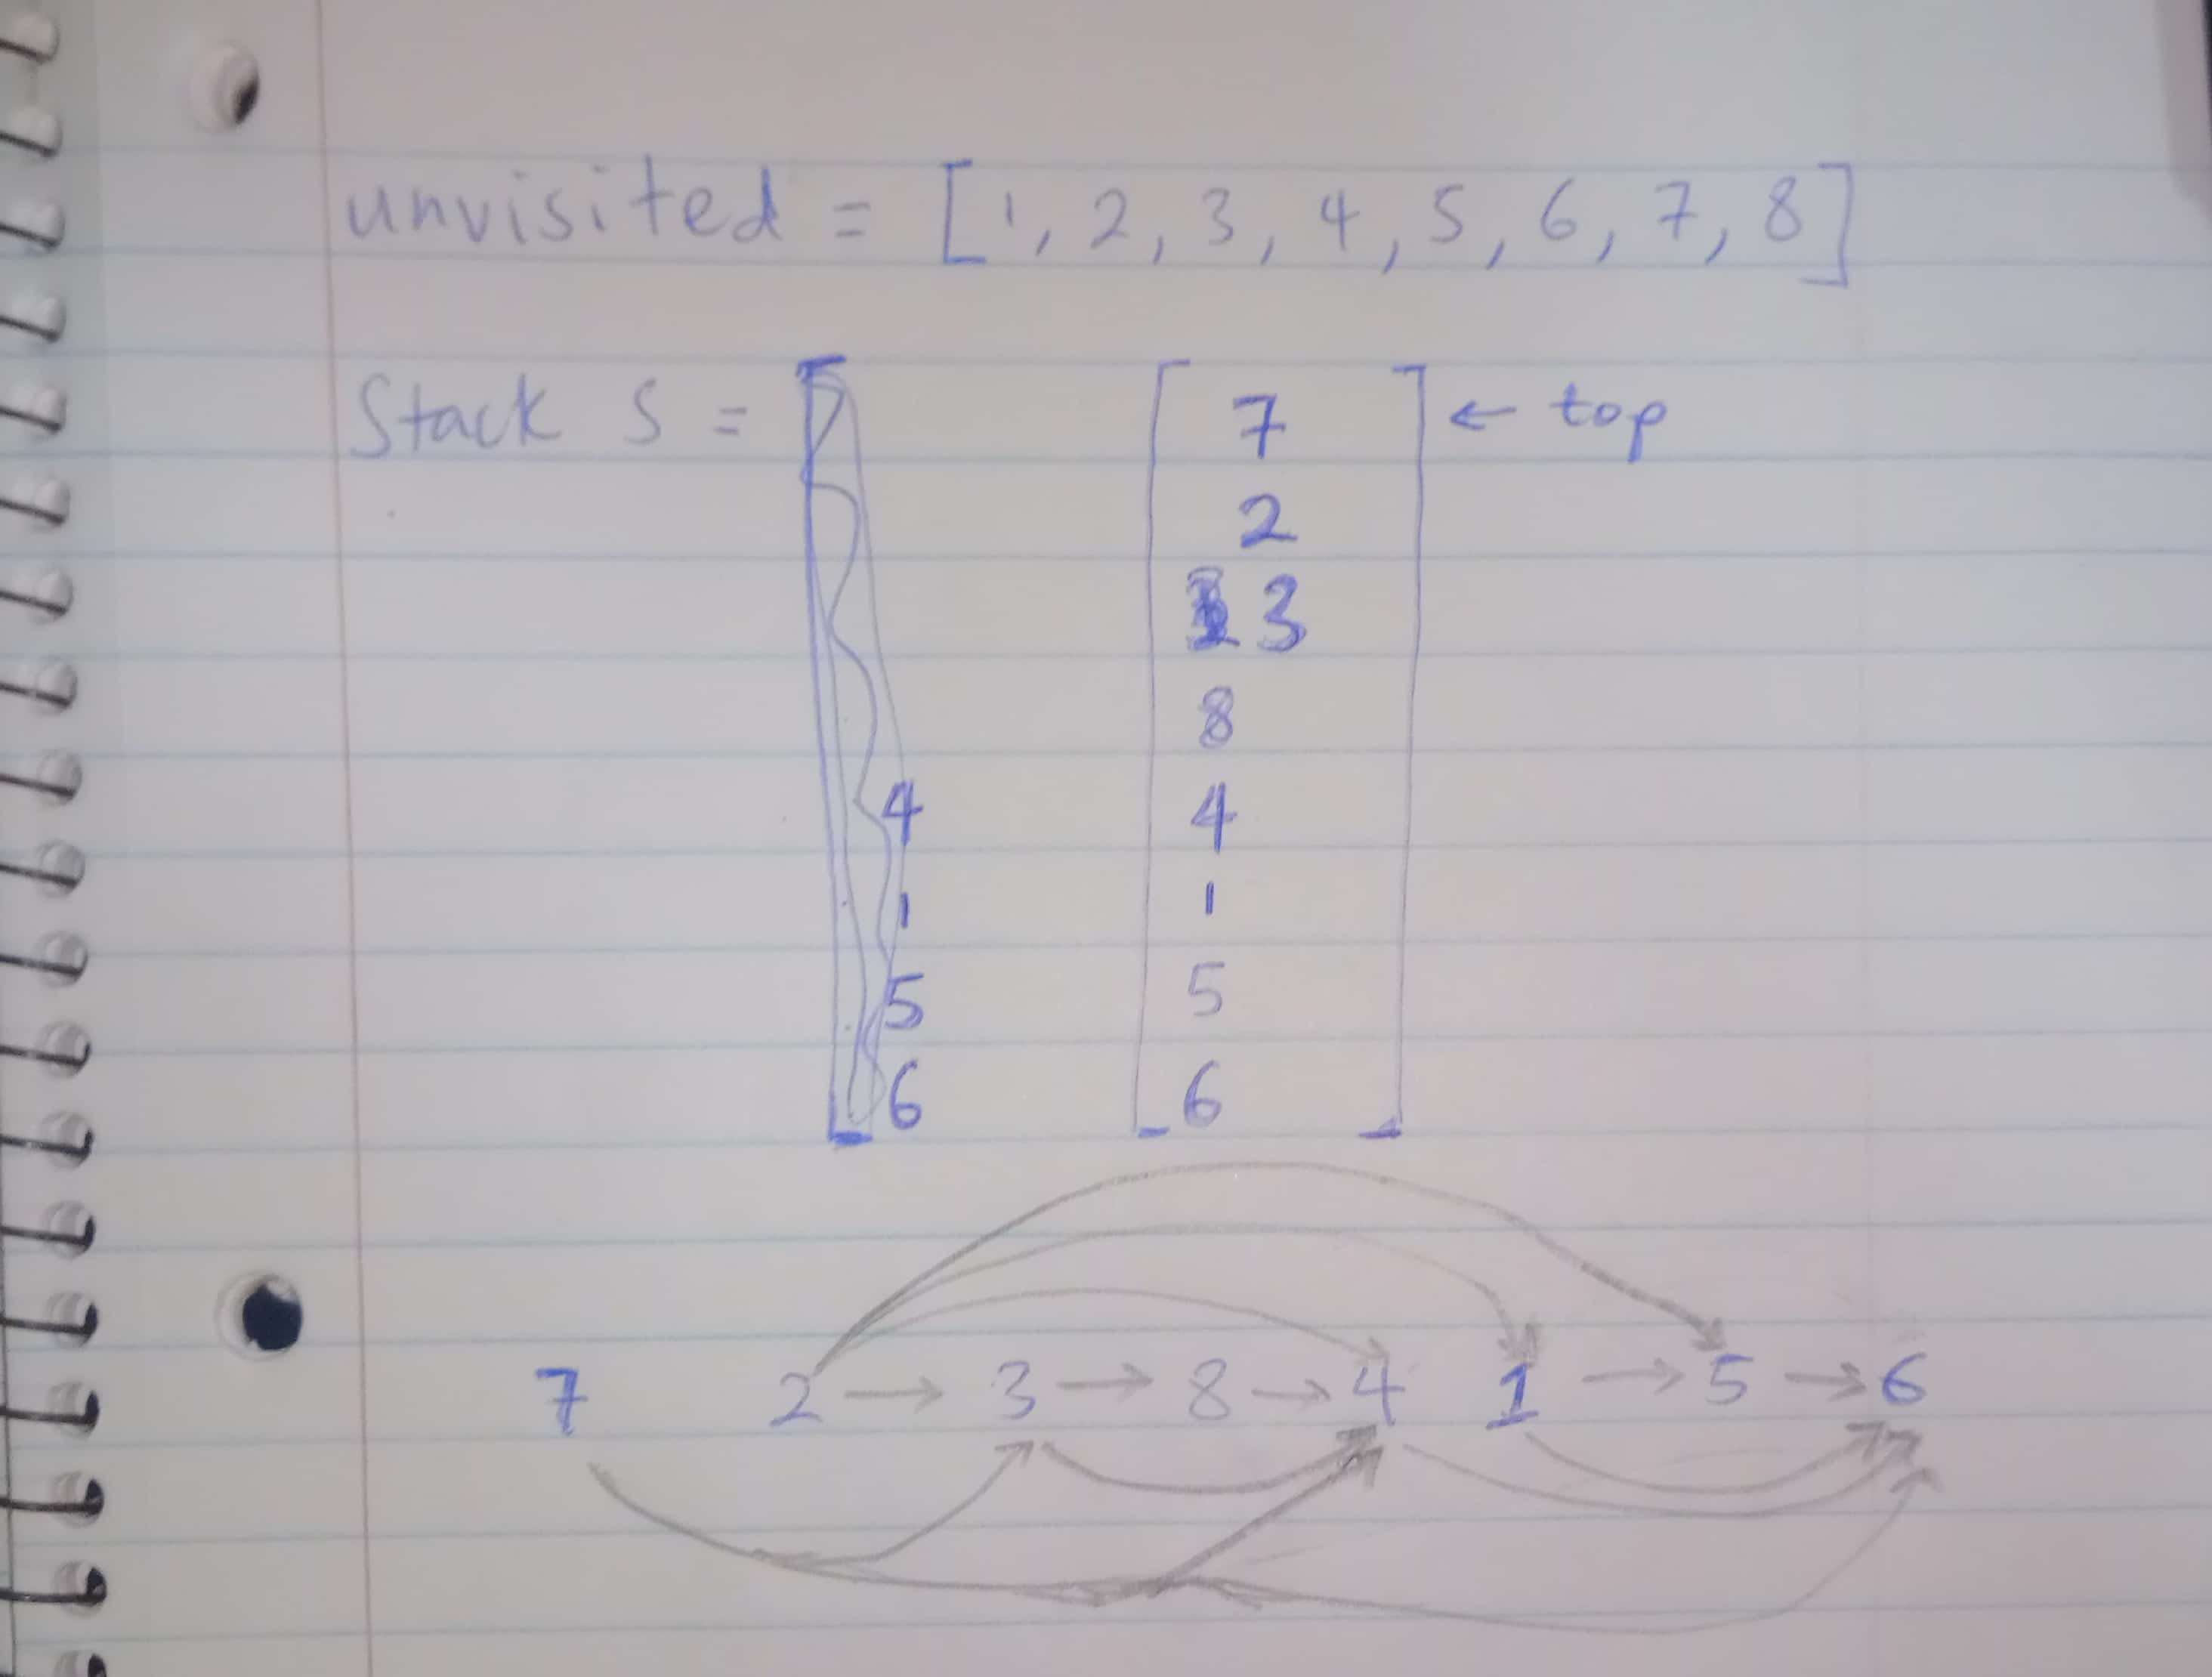
\includegraphics[width=0.8\textwidth]{tobosort23feb.jpg}
    \label{fig:topological-sort-using-dfs}
    \caption{Topological Sort Using DFS}
\end{figure}
\newpage
\subsection*{c}
\begin{figure}
    \centering
    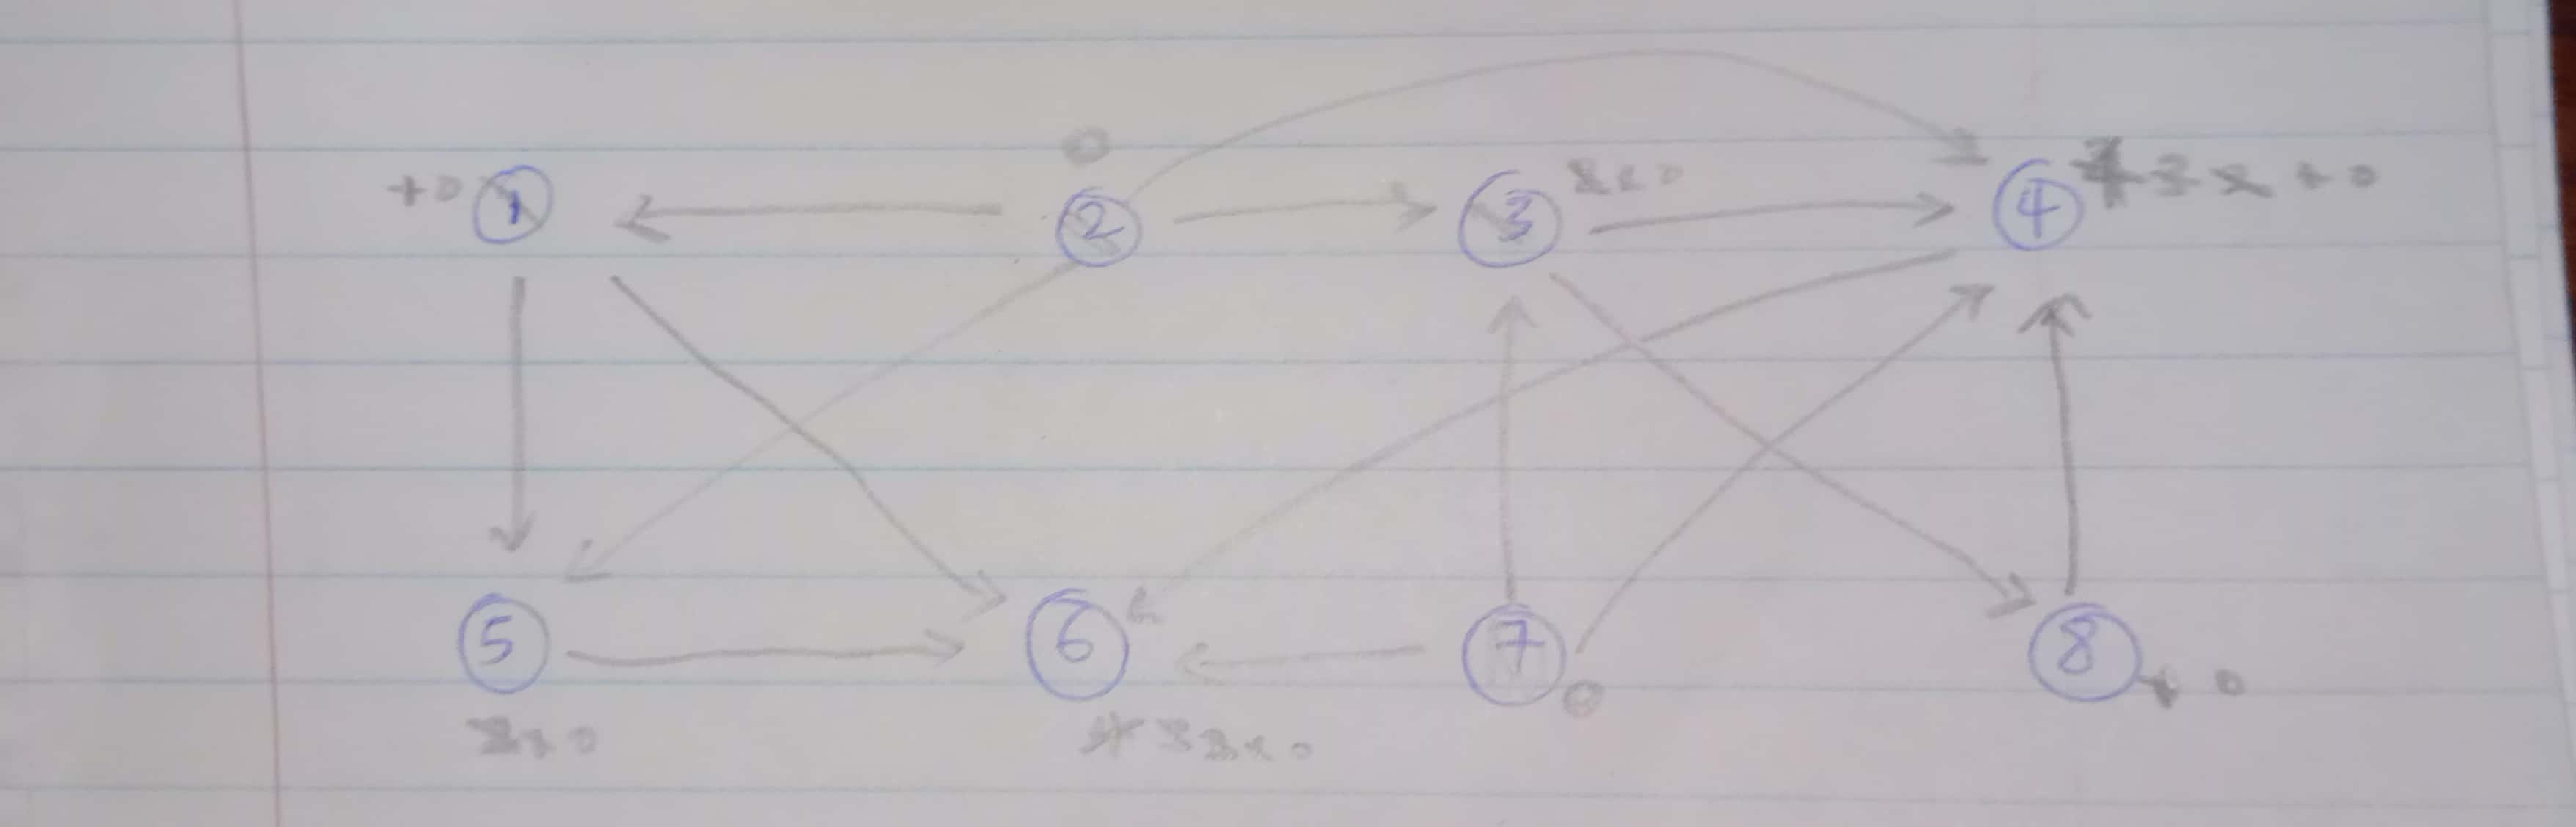
\includegraphics[width=0.8\textwidth]{sourceremoval.jpg}
    \label{fig:source-removal}
    \caption{Source Removal}
\end{figure}

\begin{figure}
    \centering
    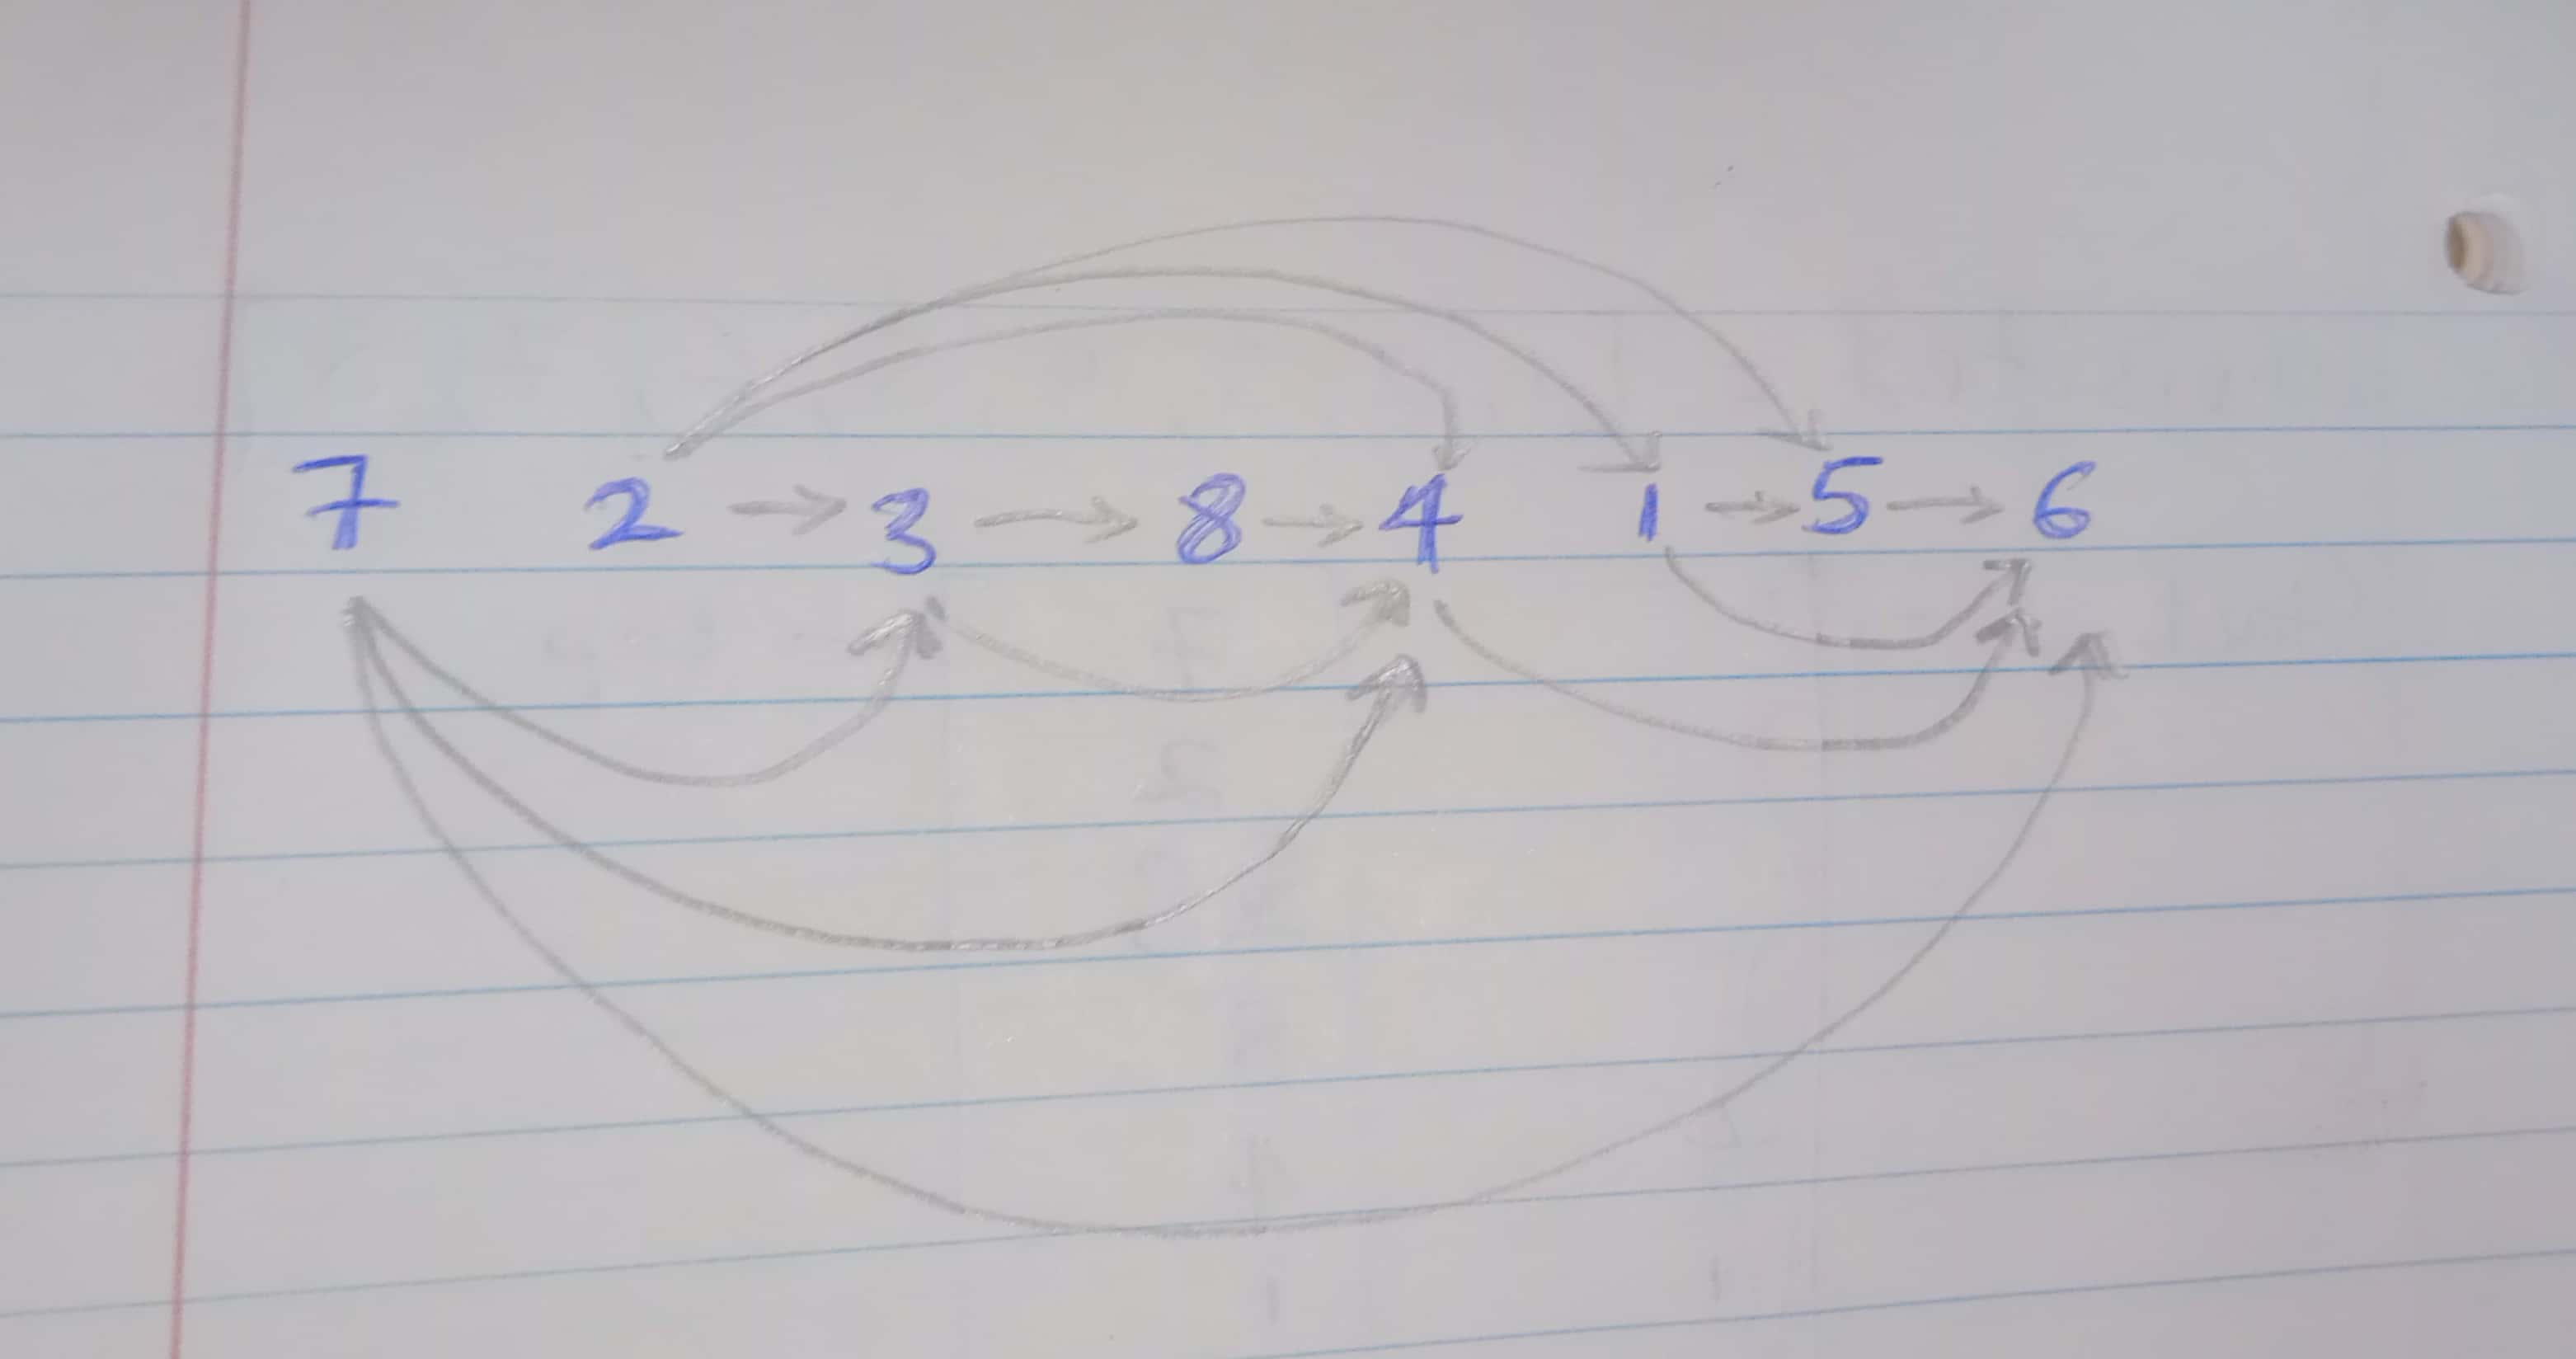
\includegraphics[width=0.8\textwidth]{tobosort23febsourcerenoval.jpg}
    \label{fig:topological-sort-source-removal}
    \caption{Topological Sort with Source Removal}
\end{figure}

\newpage
\subsection*{d}
\begin{enumerate}
    \item Initialization:
          \begin{itemize}
              \item Start with an empty list to store the topological order of vertices.
              \item Identify all source vertices in the DAG. These are vertices with no incoming edges.
          \end{itemize}

    \item Source Removal:
          \begin{itemize}
              \item While there are source vertices remaining in the DAG:
                    \begin{itemize}
                        \item Select a source vertex from the remaining source vertices.
                        \item Remove the selected source vertex from the graph.
                        \item Update the remaining source vertices (i.e., vertices that become sources after the removal of the selected vertex).
                        \item Add the selected source vertex to the topological order list.
                    \end{itemize}
          \end{itemize}

    \item Completion:
          \begin{itemize}
              \item After removing all source vertices, the topological order list contains the vertices in a valid topological order.
          \end{itemize}

    \item Output:
          \begin{itemize}
              \item Return the obtained topological order list.
          \end{itemize}
\end{enumerate}
\subsection*{e}
25 TopoSorts can be obtained from the given graph. The following are 25 possible topological orderings of the vertices in the graph:
\BlankLine
\begin{center}
    \begin{enumerate}
        \renewcommand{\labelenumi}{TopoSort\arabic{enumi}:}
        \item [TopoSort1] [2, 1, 5, 7, 3, 8, 4, 6]
        \item [TopoSort2] [2, 1, 7, 3, 8, 4, 5, 6]
        \item [TopoSort3] [2, 1, 7, 3, 8, 5, 4, 6]
        \item [TopoSort4] [2, 1, 7, 3, 5, 8, 4, 6]
        \item [TopoSort5] [2, 1, 7, 5, 3, 8, 4, 6]
        \item [TopoSort6] [2, 7, 1, 3, 8, 4, 5, 6]
        \item [TopoSort7] [2, 7, 1, 3, 8, 5, 4, 6]
        \item [TopoSort8] [2, 7, 1, 3, 5, 8, 4, 6]
        \item [TopoSort9] [2, 7, 1, 5, 3, 8, 4, 6]
        \item [TopoSort10] [2, 7, 3, 1, 8, 4, 5, 6]
        \item [TopoSort11] [2, 7, 3, 1, 8, 5, 4, 6]
        \item [TopoSort12] [2, 7, 3, 1, 5, 8, 4, 6]
        \item [TopoSort13] [2, 7, 3, 8, 1, 4, 5, 6]
        \item [TopoSort14] [2, 7, 3, 8, 1, 5, 4, 6]
        \item [TopoSort15] [2, 7, 3, 8, 4, 1, 5, 6]
        \item [TopoSort16] [7, 2, 1, 3, 8, 4, 5, 6]
        \item [TopoSort17] [7, 2, 1, 3, 8, 5, 4, 6]
        \item [TopoSort18] [7, 2, 1, 3, 5, 8, 4, 6]
        \item [TopoSort19] [7, 2, 1, 5, 3, 8, 4, 6]
        \item [TopoSort20] [7, 2, 3, 1, 8, 4, 5, 6]
        \item [TopoSort21] [7, 2, 3, 1, 8, 5, 4, 6]
        \item [TopoSort22] [7, 2, 3, 1, 5, 8, 4, 6]
        \item [TopoSort23] [7, 2, 3, 8, 1, 4, 5, 6]
        \item [TopoSort24] [7, 2, 3, 8, 1, 5, 4, 6]
        \item [TopoSort25] [7, 2, 3, 8, 4, 1, 5, 6]
    \end{enumerate}
\end{center}
\newpage
\section*{Question 5}
\begin{enumerate}
    \item Base Cases:
          \begin{itemize}
              \item If the tree is empty, return 0 (no levels).
              \item If the tree has only one node, return 1 (one level).
          \end{itemize}

    \item Divide:
          \begin{itemize}
              \item Divide the binary tree into its left and right subtrees.
          \end{itemize}

    \item Conquer:
          \begin{itemize}
              \item Recursively compute the number of levels in the left and right subtrees.
          \end{itemize}

    \item Combine:
          \begin{itemize}
              \item The number of levels in the entire tree is the maximum of the number of levels in its left and right subtrees plus one (to account for the current level).
          \end{itemize}
\end{enumerate}

\begin{verbatim}
function computeLevels(tree):
    if tree is empty:
        return 0
    else if tree has only one node:
        return 1
    else:
        leftLevels = computeLevels(left subtree of tree)
        rightLevels = computeLevels(right subtree of tree)
        return max(leftLevels, rightLevels) + 1
\end{verbatim}
Time Complexity:
\\\\The time complexity of this divide-and-conquer algorithm for computing the number of levels in a binary tree can be analyzed as follows:

\begin{itemize}
    \item At each level of recursion, the algorithm divides the problem into two subproblems (left and right subtrees) and conquers each subproblem.
    \item The recurrence relation for the time complexity is \(T(n) = 2T(n/2) + O(1)\), where \(n\) is the number of nodes in the binary tree.
    \item \[ A = 2, B = 2, k = 0, p = 0, and A > b^{k}\]
    \item Using Master Theorem, the efficiency class of the algorithm is \(\Theta(n^{log_2(2)} = \Theta(n))\).
\end{itemize}
Therefore, the time efficiency class of this algorithm is \(O(n)\),
\\where \(n\) is the number of nodes in the binary tree.
\newpage
\section*{Question 6}
\begin{enumerate}
    \item[(a)] For the recurrence relation \(T(n) = 100T(n^{1/10}) + 100(\log n)^2\), a change of variables is needed to solve:

          \begin{itemize}
              \item Let \(n = 2^m\). Then, the recurrence becomes:

                    \[T(2^m) = 100T(2^{m/10}) + 100m^2\]

              \item Let \(S(m) = T(2^m)\). Thus, the recurrence becomes:

                    \[S(m) = 100S(m/10) + 100m^2\]

              \item This is of the form \(S(m) = aS(m/b) + f(m)\). The solution is:

                    \[S(m) = O(m^2)\]

              \item Substituting back the original variables, the solution is:

                    \[T(n) = T(2^m) = S(m) = O((\log n)^2)\]
          \end{itemize}

    \item[(b)] Considering the recurrence relation \(T(n) = 7T(n/8) + n \ln n\), using Master Theorem to solve:

          \begin{itemize}
              \item Given \(a = 7\), \(b = 8\), \(k = 1\), \(p = 1\), and \(A < B^k\) and \(f(n) = n \ln n\), as \(f(n) = O(n^{k} \log^p n)\) for \(k = 1\), Master Theorem applies. Hence, the solution is:

                    \[T(n) = O(n \log n)\]
          \end{itemize}

    \item[(c)] In the recurrence relation \(T(n) = 9T(n/3) + n^2 \log n\), using Master Theorem to solve:

          \begin{itemize}
              \item Given \(a = 9\), \(b = 3\), \(k = 2\), \(p = 1\), and \(f(n) = n^2 \log n\), and \(f(n) = O(n^{\log_b a} \log^{p+1} n)\) for \(k = 1\), The solution is:

                    \[T(n) = O(n^2 \log^2 n)\]
          \end{itemize}

    \item[(d)] For the recurrence relation \(T(n) = T(n^{1/10}) + T(n^{1/5} + 2) + T(n^{1/4}) + \log n\).

\end{enumerate}
\newpage
\section*{Question 7}
\newpage
\section*{Question 8}
Explanation of how the function works:

\begin{enumerate}
    \item Base Case:
          \begin{itemize}
              \item If the length of the input array is less than 2, indicating either an empty array or an array with only one element, the function returns 0 since there are no elements to compare.
          \end{itemize}

    \item Divide:
          \begin{itemize}
              \item The function divides the input array into two equal halves.
          \end{itemize}

    \item Conquer:
          \begin{itemize}
              \item It recursively calls itself on each half of the input array to compute the maximum difference within each half.
          \end{itemize}

    \item Combine:
          \begin{itemize}
              \item The function then combines the results from the left and right halves to determine the maximum difference across the entire array.
              \item It calculates the maximum difference as the maximum of three values:
                    \begin{itemize}
                        \item The maximum difference computed from the left half.
                        \item The maximum difference computed from the right half.
                        \item The difference between the maximum and minimum values in the entire array.
                    \end{itemize}
          \end{itemize}

    \item Return Result:
          \begin{itemize}
              \item Finally, the function returns the maximum difference computed.
          \end{itemize}
\end{enumerate}
The time complexity of the \texttt{max\_difference} function can be analyzed using a recurrence relation. The recurrence relation is \(T(n) = 2 \cdot T\left(\frac{n}{2}\right) + O(1)\), where \(n\) is the size of the input array.

\begin{itemize}
    \item At each recursive call, the function divides the input array into two equal halves, resulting in \(O(1)\) time complexity for each division.
    \item The function then recursively calls itself on each half, resulting in \(2 \cdot T\left(\frac{n}{2}\right)\) time complexity for combining the results from the left and right halves.
    \item Additionally, finding the minimum and maximum values in the input array using the \texttt{min} and \texttt{max} functions also takes constant time, denoted as \(O(1)\).
\end{itemize}
Using the Master Theorem, the time complexity of the \texttt{max\_difference} function is \(O(n)\), where \(n\) is the size of the input array. This is because the time complexity of the function falls into case \( A > B^{k}\) of the Master Theorem, where \(a = 2\), \(b = 2\), \(k = 0\) and \(p = 0\), resulting in a time complexity of \(O(n^{\log_b a}) = O(n^1) = O(n)\).
\\\\Therefore, the \texttt{max\_difference} function computes the maximum difference between any two elements in an input array with a time complexity of \(O(n)\).

\end{document}